\documentclass[mathserif,handout]{beamer}
%\documentclass{beamer}
\usetheme{Warsaw}
\usecolortheme{seahorse}
\usecolortheme{orchid}
\usepackage{amsmath,verbatim}
\usepackage{listings}
\usepackage[english]{babel}
\usepackage{movie15}
\setbeamercovered{transparent}

\newcommand{\Deltap}{\ensuremath{\Delta^{\!+}}}
\newcommand{\trans}{\ensuremath{{}^\mathrm{T}}}
\newcommand{\eps}{\varepsilon}
\newcommand{\ex}[1]{{\operatorname{E}\left[#1\right]}}
\newcommand{\var}[1]{{\operatorname{Var}\left[#1\right]}}
\newcommand*{\approxdist}{\mathrel{\vcenter{\offinterlineskip
\vskip-.25ex\hbox{\hskip.55ex$\cdot$}\vskip-.25ex\hbox{$\sim$}
\vskip-.5ex\hbox{\hskip.55ex$\cdot$}}}}

% \lstMakeShortInline[language=myR]�

\lstdefinelanguage{myR} 
{
   language=R,
   otherkeywords={read.table, set.seed, head},
   deletekeywords={url,codes, t, dt, Call, formula,Q, R, on,by,hat,is,
col, set,start,end,deltat,zip},
   sensitive=true,
   breaklines=true,
   morecomment=[l]{\#},
   morestring=[b]",
   morestring=[b]',
   basicstyle =\ttfamily\small,
   keywordstyle=\bfseries,
   showtabs=false,
   showstringspaces=false,
   literate= {~}{$\sim$}{2},
   numberstyle=\sffamily\scriptsize,
   stepnumber=2
 }




\title[An introduction to computer models]{A tutorial introduction to the analysis of complex computer models}
\author[Darren Wilkinson --- NUFEB, 3/6/2014]{\textbf{\large Darren 
Wilkinson} \\
\alert{\url{http://tinyurl.com/darrenjw}}\\
School of Mathematics \& Statistics, \\
Newcastle University, UK}
\date{NUFEB Seminar\\Newcastle University\\3rd June, 2014}

\begin{document}

\section{Introduction}

\frame{\titlepage}

\subsection{Overview}

\frame{
\frametitle{About this presentation...}
\begin{itemize}
\item This talk is written using the \LaTeX\ documentation preparation system (\url{http://www.latex-project.org/})
\item All computations and figures were produced using the R statistical programming language (\url{http://www.r-project.org/})
\item The \LaTeX\ source code for the talk and the R scripts for carrying out all computations and generating the figures are in the NUFEB GitHub repository in the directory \url{LargeScaleModelling/Darren/Talks/ComputerModels}
\item There is a \texttt{Makefile} in the directory which can be used for generating all plots and compiling the PDF of this presentation using GNU Make (\url{http://www.gnu.org/software/make/})
\end{itemize}
}

\frame{
\frametitle{What to talk about?}
NUFEB brings together a large number of my research interests, so there are lots of different things that I \emph{could} have talked about today...
\begin{itemize}
\item Noise, stochasticity and heterogeneity in biological systems
\item Stochastic computational modelling in systems biology
\item Multiscale stochastic modelling
\item Bayesian parameter estimation for complex stochastic biological models
\item Bayesian network modelling
\item Bayesian hierarchical statistical modelling of large and complex high-throughput experimental data
\item \alert{The design and analysis of complex computer models}
\end{itemize}
}

\frame{
\frametitle{Overview}
\begin{itemize}
\item Complex computer models
\item Emulation of a computer model (using Gaussian processes)
\item The design of computer experiments
\item Confronting reality: history matching
\item Calibration/parameter estimation
\item Model discrepancy versus measurement error --- estimating the \emph{bias} term
\item Bayesian inference...
\end{itemize}

The main aim of the talk today is to get people to understand what these words mean!
}


\subsection{Computer models and emulators}

\frame{
\frametitle{Computer models}
\begin{itemize}
\item The ultimate goal of NUFEB is to develop techniques for building computer models of real, complex physical systems, and for using such models to better understand how to control and manipulate real systems with minimal physical experimentation
\item Computer models are \alert{simulators} --- they represent the physical system, and can be used to predict the behaviour of a physical system under varying scenarios
\item To be useful, it must be quicker, easier and cheaper to run the computer model for a given scenario than to perform a physical experiment, and they must also be a sufficiently good representation of reality
\item However, complex models can be computationally \alert{expensive}, often taking hours or days to perform a single run for a single given scenario
\end{itemize}
}

\frame{
\frametitle{Computer experiments}
\begin{itemize}
\item Due to the expense of running complex codes, it is necessary to carefully \alert{design experiments} for computer models, somewhat analogous to physical designed experiments
\item Just as we perform real experiments to reduce our uncertainty about the behaviour of physical systems, we can perform experiments on computer models to reduce our uncertainty about their (pre-determined, but unknown) behaviour
\item Computer models often have various \alert{input parameters}, which we denote by $\mathbf{x}$, which alter the behaviour of the computer model
\item Models will often generate lots of output. For this talk, we will consider a \alert{single output} of primary interest, $y$, which is a \alert{deterministic} function of the inputs (even if there is some \alert{stochasticity} internal to the computer model)
\end{itemize}
}

\frame{
\frametitle{Model inputs: control variables}
\begin{itemize}
\item \alert{Control variables}, often $\mathbf{x}$ or $\mathbf{x}_c$, are present in both the computer model and the corresponding physical system, and can be set by the engineer to control the product or process
\item Examples relevant to bioreactors include the recycling ratio, purge ratio, dissolved oxygen content (controlled by aeration), etc.
\end{itemize}
}

\frame{
\frametitle{Model inputs: environmental variables}
\begin{itemize}
\item \alert{Environmental variables}, often $\mathbf{x}_e$, like control variables, are also present in both the physical system and the computer model, but in the physical system they are outside the control of the engineer
\item Sometimes confusingly referred to as ``noise" variables
\item Examples relevant to bioreactors include the composition of the incoming raw sewage and water temperature
\end{itemize}
}

\frame{
\frametitle{Model inputs: model variables}
\begin{itemize}
\item \alert{Model variables} or \alert{model parameters}, often $\boldsymbol{\theta}$ or $\mathbf{x}_m$, don't really exist in the physical system, but are considered to have some ``true" or ``best" setting, initially unknown, which makes the simulator match reality as well as possible
\item Sometimes referred to as \alert{tuning parameters}
\item Much controversy about the existence and interpretation of model parameters corresponding to constants with a physical interpretation which could in principle be measured (\emph{in vitro} if not \emph{in vivo})
\item Due to inadequacy of a model, it may behave better when parameters with a physical interpretation are tuned to non-physical values (cf. climate models)
\item Examples relevant to bioreactors include rates of biochemical process, rates of cellular processes, viscosity of water, adhesive strength of a particular biofilm, etc.
\end{itemize}
}

\frame{
\frametitle{Model output}
\begin{itemize}
\item \alert{Output}, often $y$, is a key (deterministic) system output of interest, corresponding to something measurable on the physical system being modelled
\item Although simulation models often generate large amounts of output, there are often a relatively small number of outputs of main interest corresponding to measurable quantities on the corresponding physical system
\item This talk will focus on a single output --- extensions to multiple outputs are well studied
\item Examples relevant to bioreactors include output BOD, output COD, heterotroph fraction, average floc size, ammonia concentration, etc.
\item The simulator maps inputs $\mathbf{x}$ deterministically to output $y$, and can therefore be considered a \alert{function}, $f(\cdot)$, governing the mapping $y=f(\mathbf{x})$, which is expensive to evaluate
\end{itemize}
}

\frame{
\frametitle{A multi-scale model of a bioreactor}
\begin{itemize}
\item Let's jump \alert{forward in time two years}...
\item We've appointed a modeller and we've built the most ambitious and realistic multiscale model of a bioreactor ever attempted (hurray!!!)
\item We've worked hard to make the code as efficient as we can, and it now takes just 24 hours to do a single run of the code for a single set of model inputs on our computer cluster
\item Although there is stochasticity in the model, our key output of interest is a long run average of a stationary quantity (say, BOD), which can be considered to be deterministic
\item However, there's one model parameter that we aren't too sure about how to set...
\end{itemize}
}

\frame{
\frametitle{Evaluating the simulator at multiple inputs}
\centerline{\includegraphics[height=0.9\textheight]{sim1}}
}

\frame{
\frametitle{Evaluating the simulator at multiple inputs}
\centerline{\includegraphics[height=0.9\textheight]{sim2}}
}

\frame{
\frametitle{Evaluating the simulator at multiple inputs}
\centerline{\includegraphics[height=0.9\textheight]{sim3}}
}

\frame{
\frametitle{Evaluating the simulator at multiple inputs}
\centerline{\includegraphics[height=0.9\textheight]{sim4}}
}

\frame{
\frametitle{Evaluating the simulator at multiple inputs}
\centerline{\includegraphics[height=0.9\textheight]{sim5}}
}

\frame{
\frametitle{Evaluating the simulator at multiple inputs}
\centerline{\includegraphics[height=0.9\textheight]{sim6}}
}

\frame{
\frametitle{Emulating a computer model}
\begin{itemize}
\item An \alert{emulator} is a \alert{cheap} (fast) surrogate for the computer model, which has many potential uses
\item Principally, it can be used instead of the real model in algorithms that require many evaluations of the simulator at many different input configurations
\item Some emulators are good and some are bad --- to be useful, they should have a measure of \alert{uncertainty} associated with them
\item \alert{Stochastic process} emulators define a probability distribution on the space of functions consistent with any known evaluations of the simulator
\item \alert{Gaussian processes} (GPs) are one of the simplest and most tractable stochastic processes on function space
\end{itemize}
}

\frame{
\frametitle{Sequential updating of a GP emulator}
\centerline{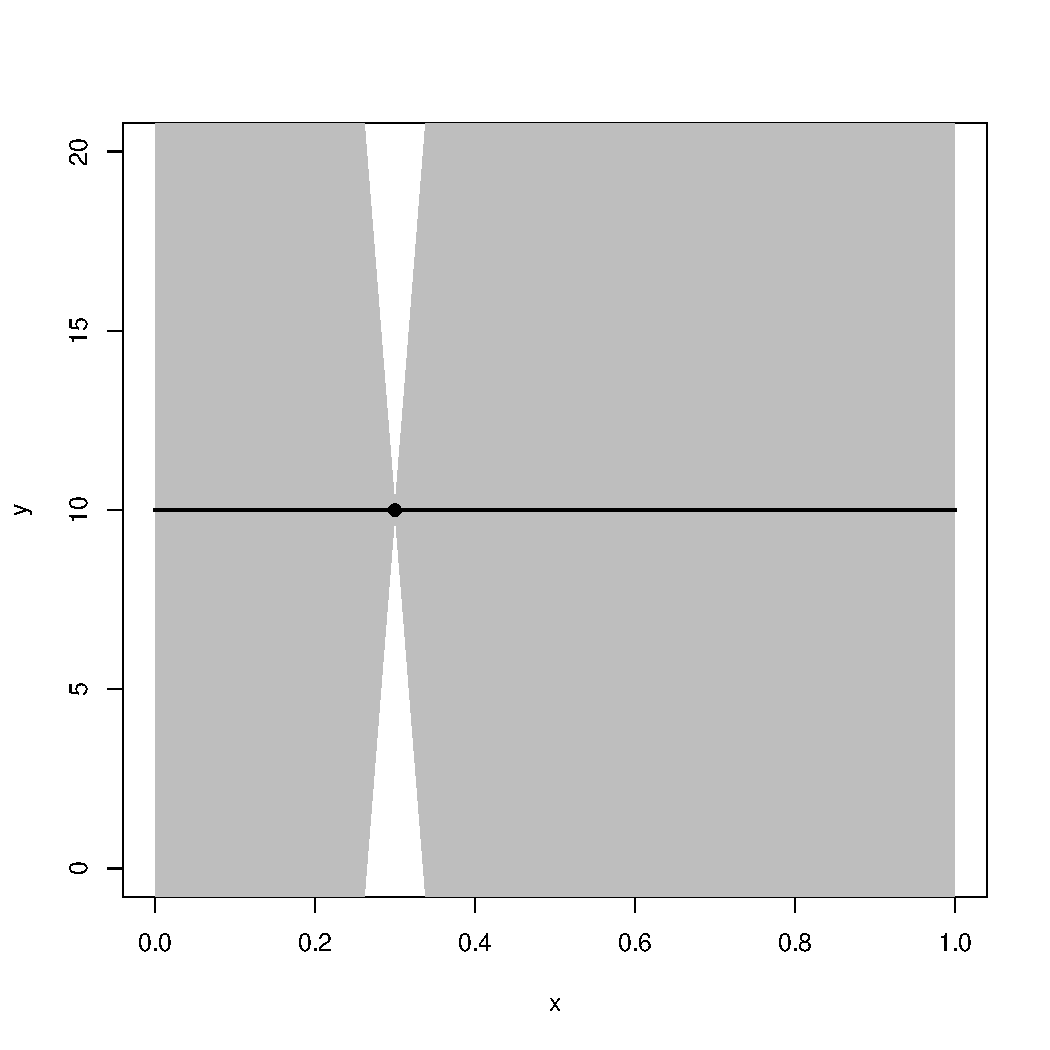
\includegraphics[height=0.9\textheight]{emu1}}
}

\frame{
\frametitle{Sequential updating of a GP emulator}
\centerline{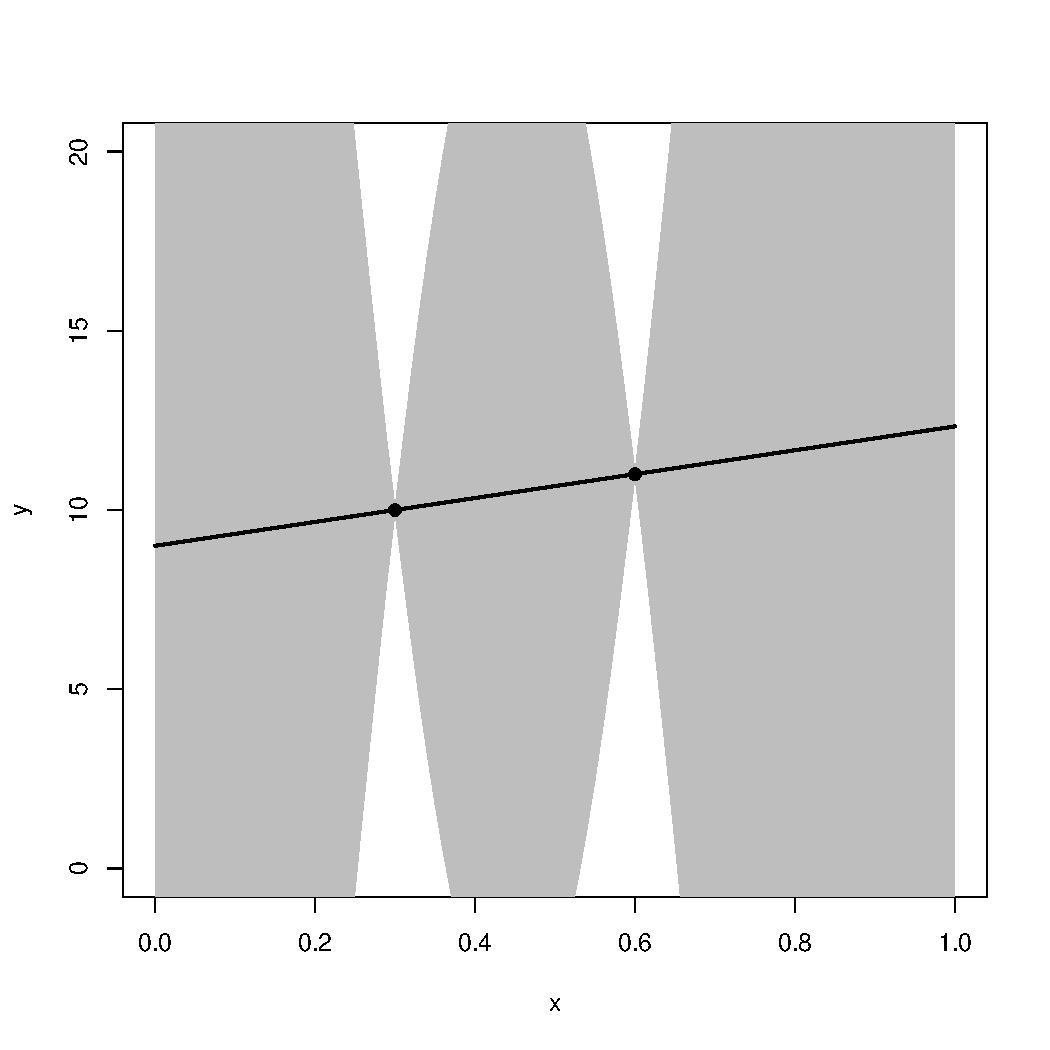
\includegraphics[height=0.9\textheight]{emu2}}
}

\frame{
\frametitle{Sequential updating of a GP emulator}
\centerline{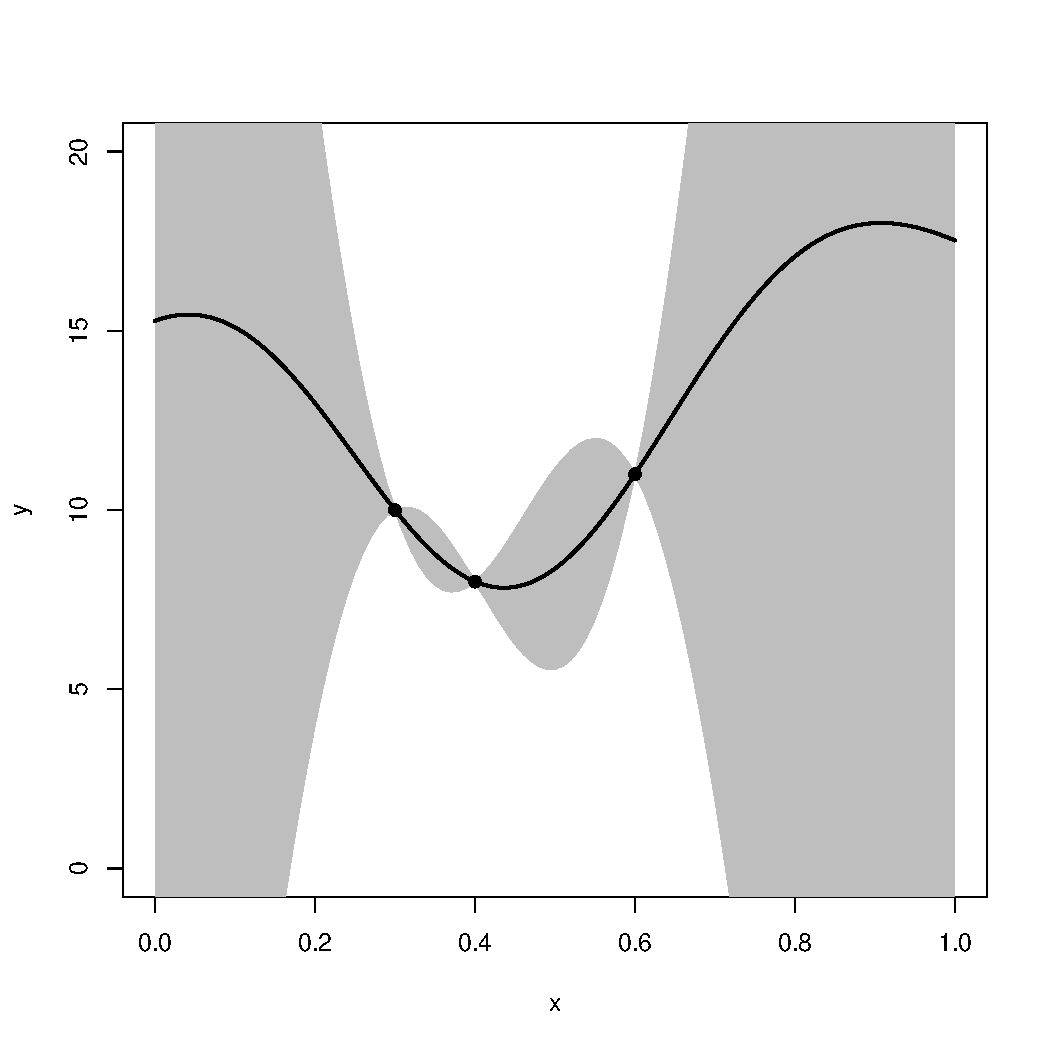
\includegraphics[height=0.9\textheight]{emu3}}
}

\frame{
\frametitle{Sequential updating of a GP emulator}
\centerline{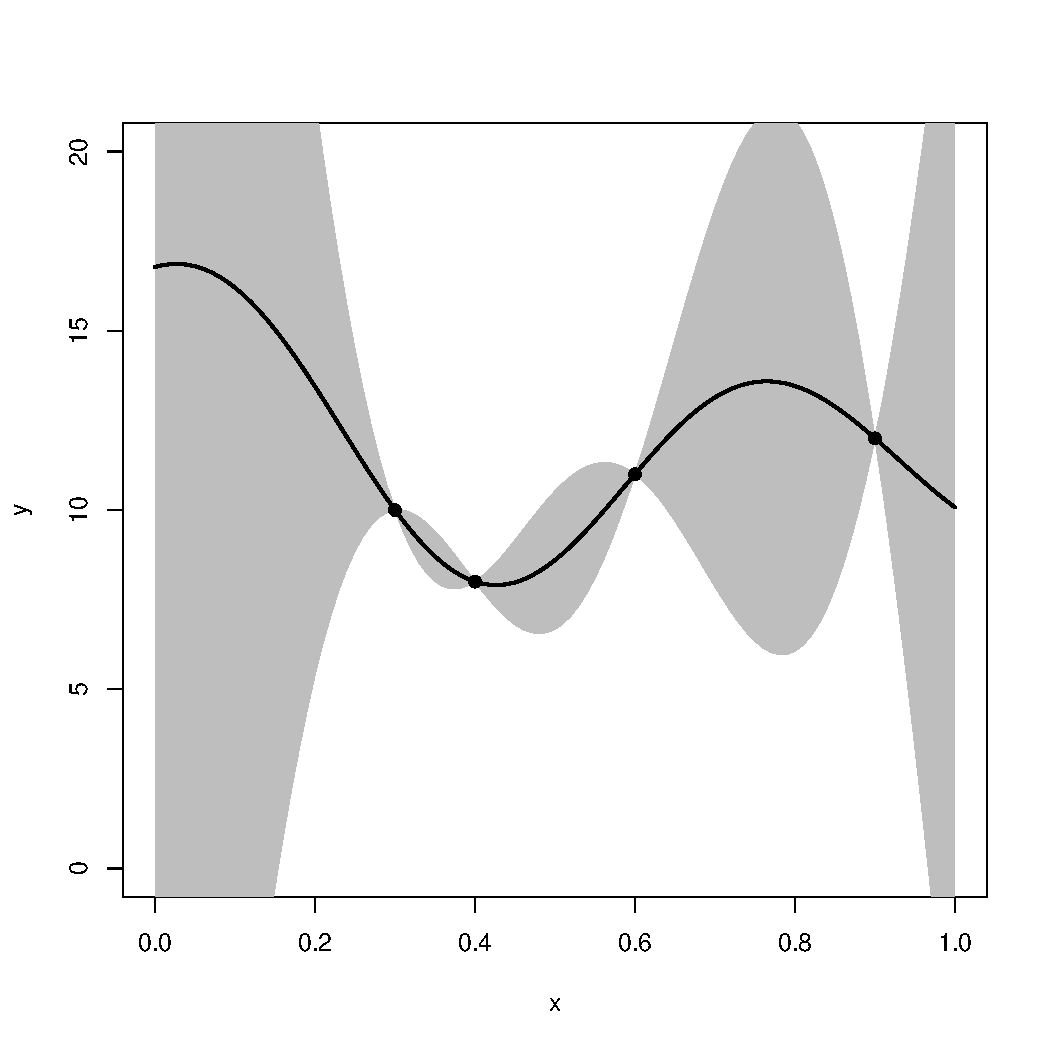
\includegraphics[height=0.9\textheight]{emu4}}
}

\frame{
\frametitle{Sequential updating of a GP emulator}
\centerline{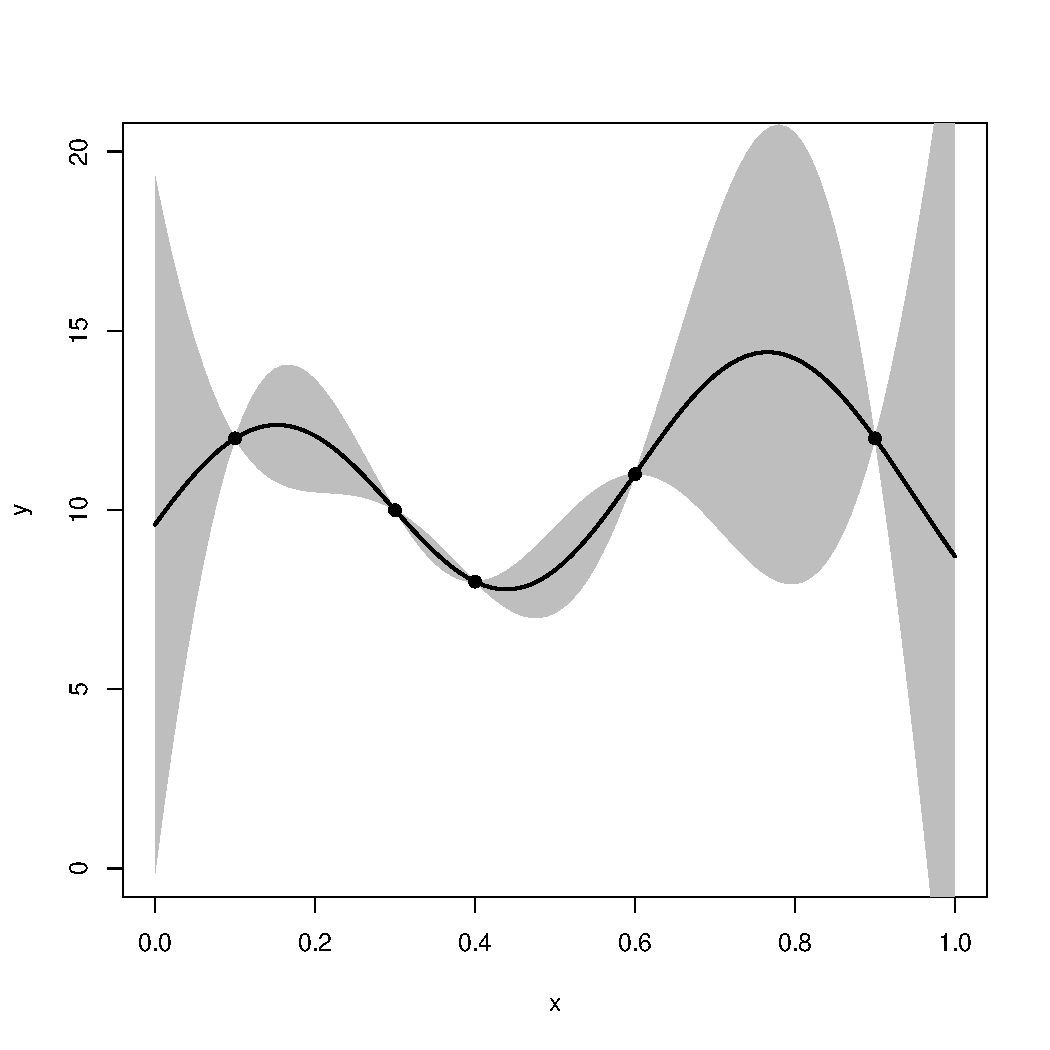
\includegraphics[height=0.9\textheight]{emu5}}
}

\frame{
\frametitle{Sequential updating of a GP emulator}
\centerline{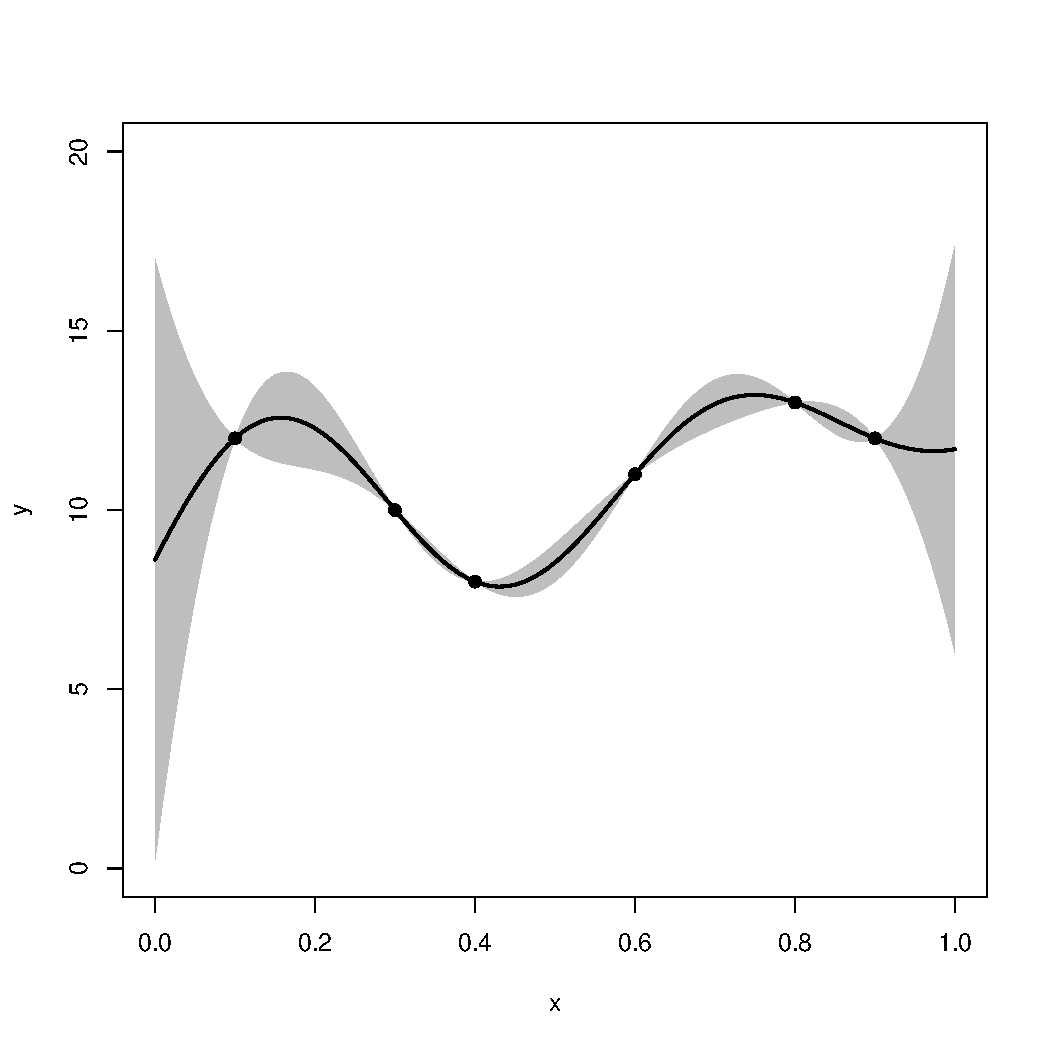
\includegraphics[height=0.9\textheight]{emu6}}
}

\frame{
\frametitle{Gaussian processes}
\begin{itemize}
\item A GP is a probability distribution on functions defined so that the marginal distribution of any finite number of points always has a multivariate normal (MVN) distribution
\item Points close together in input space are typically more highly correlated than points far away
\item Stationary GPs are defined by a \alert{covariance function} --- many different possible choices - here I've used a Gaussian kernel
\[
\operatorname{Cov}[f(\mathbf{x}),f(\mathbf{x}')] = K(\mathbf{x},\mathbf{x}') = \sigma^2\exp\left\{-\left(\frac{\Vert \mathbf{x}-\mathbf{x}'\Vert_2}{r}\right)^2\right\},
\]
containing two parameters: an asymptotic variance, $\sigma^2$, and a correlation length scale, $r$.
\item A GP conditioned on observations is also a GP (\alert{Kriging})
\end{itemize}
}

\frame{
\frametitle{Samples from a GP posterior distribution}
\centerline{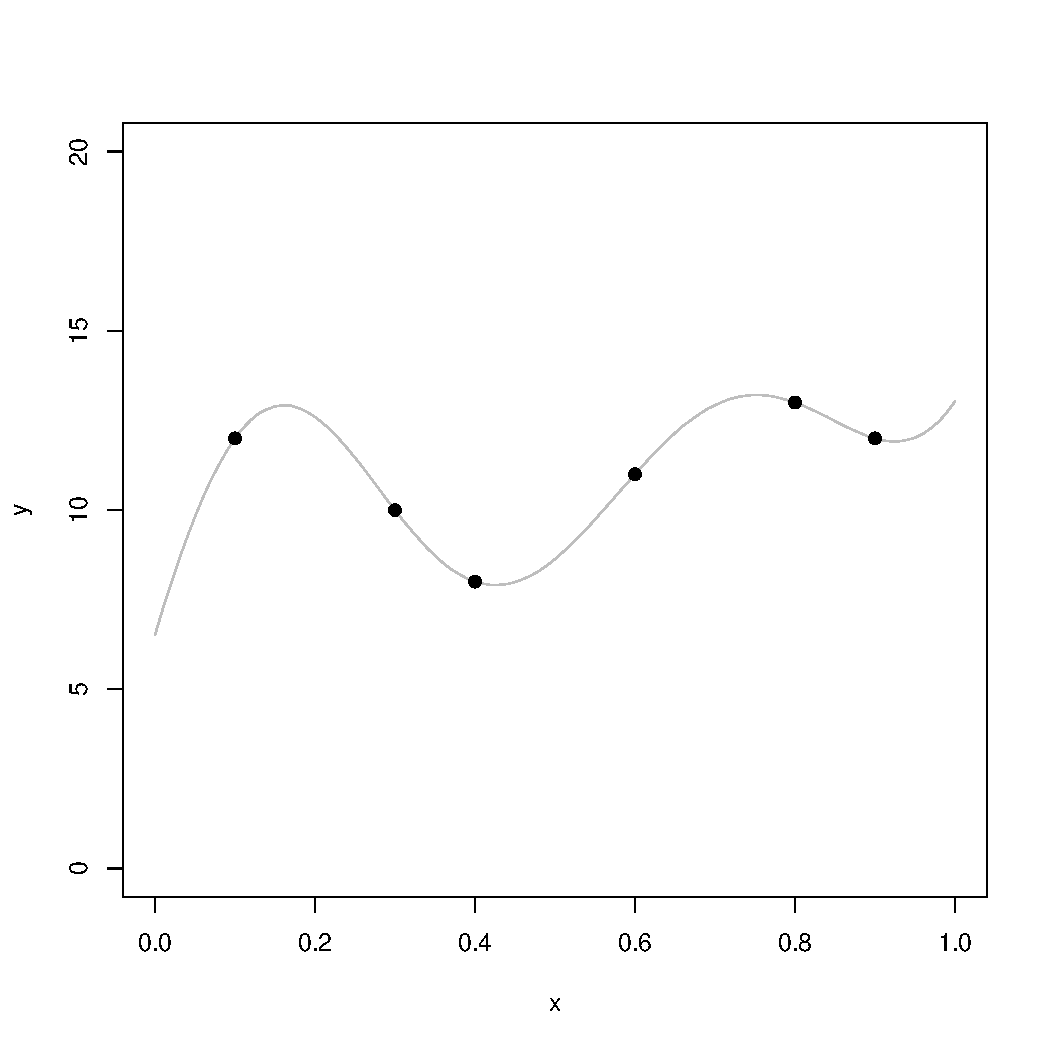
\includegraphics[height=0.9\textheight]{sample1}}
}

\frame{
\frametitle{Samples from a GP posterior distribution}
\centerline{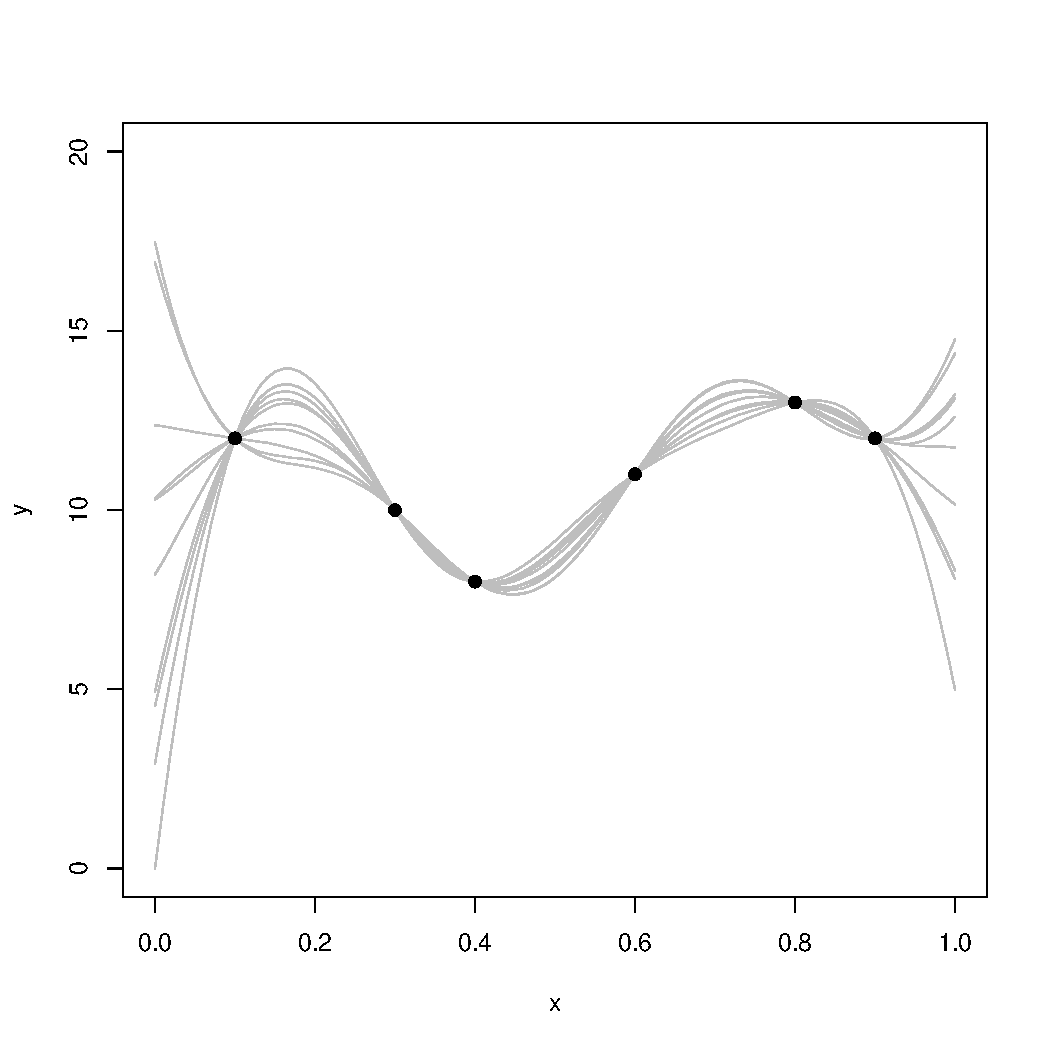
\includegraphics[height=0.9\textheight]{sample10}}
}

\frame{
\frametitle{Samples from a GP posterior distribution}
\centerline{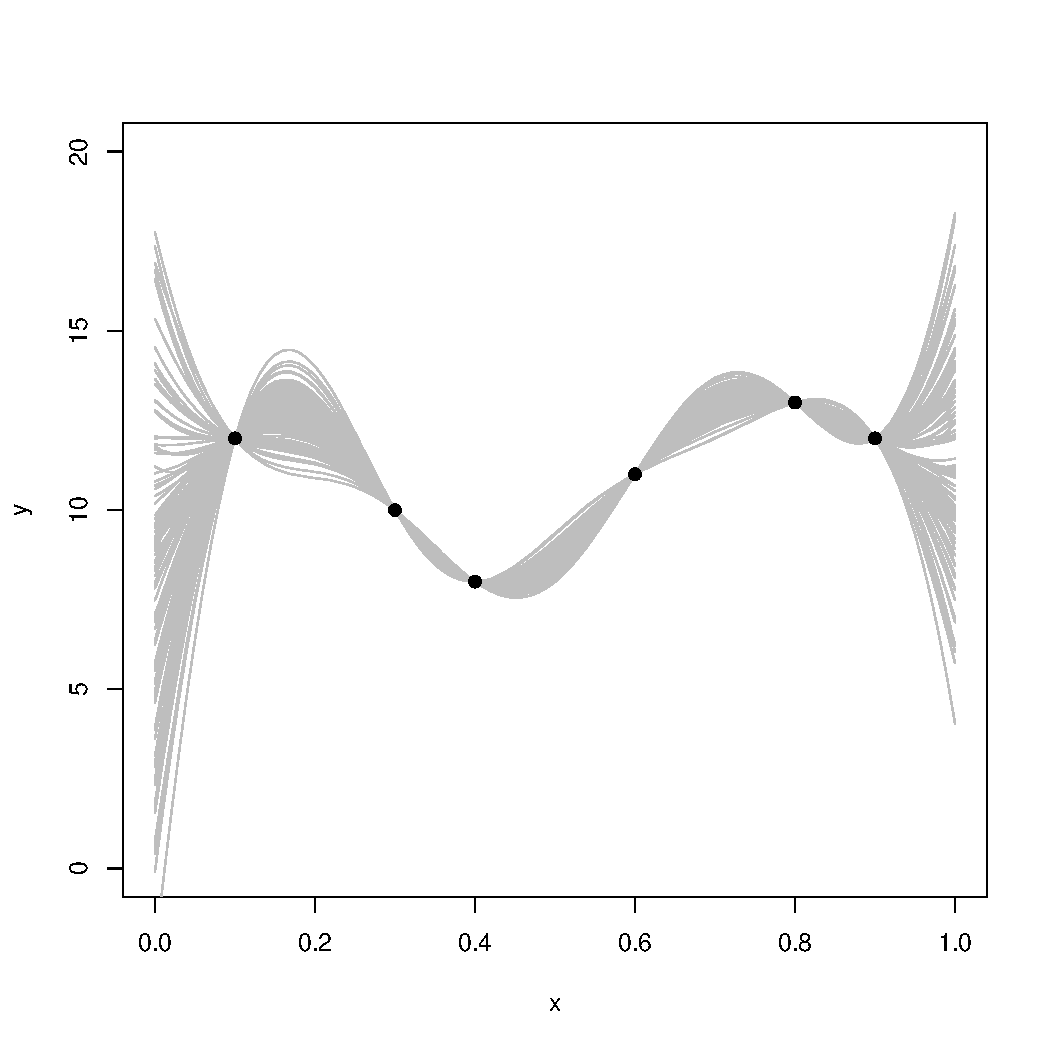
\includegraphics[height=0.9\textheight]{sample100}}
}

\subsection{Design of computer experiments}

\frame{
\frametitle{Design of computer experiments}
\begin{itemize}
\item To build a ``good" emulator, we want residual uncertainty to be small. In 1d this is easy, but in higher dimensions we need to choose \alert{design points} to \alert{fill space} efficiently so that there aren't big gaps in parameter space for which we don't have a simulator run
\item The naive approach to this problem is to construct a \alert{Cartesian product design} where many levels of each variable are considered in turn, but this approach becomes unworkable in more than 2 or 3 dimensions
\item \alert{Latin hypercube designs} (LHDs) are a good way to choose design points to fill space in an efficient way
\item In more than 2 dimensions, Cartesian product designs are a very inefficient way of covering the design space, and LHDs are much better. In other words, naive \alert{parameter scans are bad --- don't do them!}
\end{itemize}
}

\frame{
\frametitle{A 2D Latin hypercube design}
\centerline{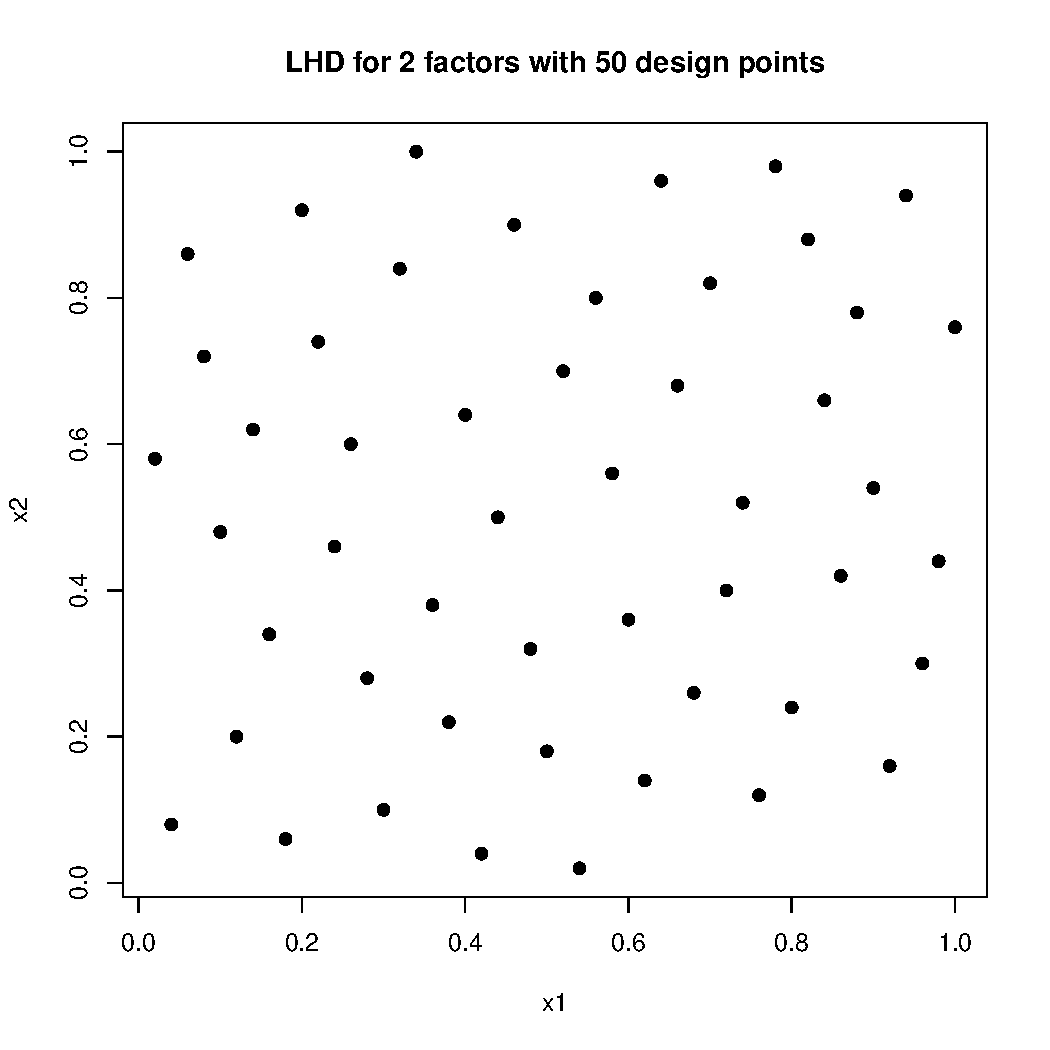
\includegraphics[height=0.9\textheight]{lhd}}
}

\section{Linking computer models to reality}

\subsection{History matching}

\frame{
\frametitle{History matching}
\begin{itemize}
\item Suppose now that we have $n$ measurements on the real physical system: $\{(z_1,\mathbf{x}_1),(z_2,\mathbf{x}_2),\ldots,(z_n,\mathbf{x}_n)\}$
\item $z_i$ is the measured value of the output variable $y$ obtained when the physical system has control parameters set to $\mathbf{x}_i$
\item Let $y(\mathbf{x})$ denote the true state of the output variable (reality) when the control parameters at set to $\mathbf{x}$
\item Then the measurements and reality are related by
\[
z_i = y(\mathbf{x}_i) + e_i,
\]
where $e_i$ is (typically, Gaussian) measurement error
\end{itemize}
}

\frame{
\frametitle{Linking the simulator to physical measurements}
\begin{itemize}
\item The computer model and reality are related by
\[
y(\mathbf{x}) = f(\mathbf{x},\boldsymbol{\theta}) + \delta(\mathbf{x}),
\]
where $\boldsymbol{\theta}$ represents the ``best" or ``true" value of the model parameters, $\boldsymbol{\theta}$, and $\delta(\mathbf{x})$ represents the \alert{discrepancy} between the simulator and reality when the control parameters are set to $\mathbf{x}$ (\alert{bias} term)
\item The measurements and the simulator are therefore related by
\[
z_i = f(\mathbf{x}_i,\boldsymbol{\theta}) + \delta(\mathbf{x}_i) + e_i
\]
\item It is tempting to lump together $\delta(\mathbf{x}_i) + e_i$ into a single source of ``error", but we will see later why this is not necessarily a good idea
\end{itemize}
}

\frame{
\frametitle{Implausibility}
\begin{itemize}
\item For most settings of the model parameters, $\boldsymbol{\theta}$, the model will be inconsistent with the observed measurements
\item Want to use emulator to rule out regions of parameter space which are \alert{implausible} (taking into account emulator uncertainty about the true simulator output)
\item Implausibility defined by
\[
I(\mathbf{x}) \equiv \frac{|\ex{f(\mathbf{x})}-z|}{\operatorname{SD}[\ex{f(\mathbf{x})}-z]} = \sqrt{\frac{(\ex{f(\mathbf{x})}-z)^2}{\var{f(\mathbf{x})}+\var{\delta(\mathbf{x})}+\var{e}}}
\]
\item Pukelsheim's three-sigma rule suggests ruling out parts of parameter space where the implausibility is larger than 3
\end{itemize}
}

\frame{
\frametitle{Implausibility plots}
\centerline{\includegraphics[height=0.9\textheight]{imp1}}
}

\frame{
\frametitle{Implausibility plots}
\centerline{\includegraphics[height=0.9\textheight]{imp2}}
}

\frame{
\frametitle{Implausibility plots}
\centerline{\includegraphics[height=0.9\textheight]{imp3}}
}

\frame{
\frametitle{Implausibility plots}
\centerline{\includegraphics[height=0.9\textheight]{imp4}}
}

\frame{
\frametitle{Implausibility plots}
\centerline{\includegraphics[height=0.9\textheight]{imp5}}
}

\frame{
\frametitle{Implausibility plots}
\centerline{\includegraphics[height=0.9\textheight]{imp6}}
}

\frame{
\frametitle{Iterative re-focussing}
\begin{itemize}
\item History matching can be used iteratively in order to efficiently develop emulators which are extremely accurate in the regions of parameter space which are most consistent with available observations of the physical system
\item An initial computer experiment can be used to build an initial emulator of a simulator over a large parameter range
\item Implausibility analysis can be used to rule out large parts of the parameter space
\item A new computer experiment can be designed on a smaller space including the region of interest
\item A new emulator can be developed based on \emph{all} available simulator runs
\item A new implausibility analysis can be carried out to rule out more regions of parameter space and the process repeated...
\end{itemize}
}

\subsection{Calibration, parameter estimation and Bayesian inference}

\frame{
\frametitle{Bayesian model calibration}
Tuning model parameters so that output from the model ``better
matches'' experimental data is a standard optimisation problem, but is
problematic and unsatisfactory for a number of reasons:
\begin{itemize}
\item Defining an appropriate ``objective function'' is not
 straightforward if the model is stochastic or the measurement error
 has a complex structure (not IID Gaussian) 
\item The statistical
 concept of \alert{likelihood} provides the ``correct'' way of
 measuring the evidence in favour of a set of model parameters, but
 typically requires computationally intensive Monte Carlo procedures
 for evaluation in complex settings 
\item Simple optimisation of the
 likelihood (the \alert{maximum likelihood} approach) is also unsatisfactory,
 as there are typically many parameter combinations with very similar
 likelihoods (and the likelihood surface is typically multi-modal,
 making global optimisation difficult)
\end{itemize}
}

\frame{
\frametitle{Markov chain Monte Carlo (MCMC)}
\begin{itemize}
\item Additionally, likelihood ignores any existing information known
about likely parameter values \emph{a priori}, which can be very
useful for regularising the inference problem --- better to base
inference on the \alert{posterior distribution}
\item \alert{MCMC algorithms} can be used to explore plausible regions of
parameter space in accordance with the posterior distribution ---
these provide rich information
\item eg. rather than simple point estimates for parameter values, can get
\alert{plausible ranges} of values, together with information on parameter
\alert{identifiability} and \alert{confounding}
\item MCMC algorithms are computationally intensive, but given that
evaluation of the likelihood is typically computationally intensive
anyway, nothing to lose and everything to gain by doing a Bayesian
analysis --- another talk...
\end{itemize}
}


\subsection{The bias term and fast simulators}

\frame{
\frametitle{Model discrepancy}
\begin{itemize}
\item Computer models are never a perfect reflection of reality --- don't ignore it --- deal with it!
\item If there are no control variables it is difficult to disentangle the model discrepancy from the measurement error, but that doesn't mean that a systematic bias should be ignored! Can still estimate the error distribution...
\item If there \emph{are} control variables, it really is worth trying to understand the discrepancy between the simulator and reality: it exists, it is important, it can be estimated, and it can be useful for understanding how to control the physical system
\item Can model the discrepancy with another GP
\item A picture can explain the basic idea...
\end{itemize}
}

\frame{
\frametitle{Model discrepancy}
\centerline{\includegraphics[height=0.9\textheight]{disc}}
}

\frame{
\frametitle{Fast simulators}
\begin{itemize}
\item Often it will be possible to speed up a simulator by coarsening grids, introducing mean field approximations, etc.
\item The \alert{fast} simulator is likely to be less accurate than the \alert{slow} simulator, but if it exhibits similar characteristics over a range of inputs then it could still be very useful, as it will be easier to obtain a large number of function evaluations
\item Just as we can make improved predictions about the real physical system by understanding the discrepancy between the simulator and experimental observations, we can also develop an improved emulator of the slow simulator by understanding the discrepancy between the slow simulator and a fast approximation for which many (more) function evaluations are available --- the principles are very similar
\end{itemize}
}


\section{Conclusion}

\subsection{Discussion}

\frame{
\frametitle{Discussion}
\begin{itemize}
\item Building large and complex computer models of a physical system is fun, interesting and challenging, but understanding the model and its relationship with the actual real system is equally challenging
\item There is a large body of Bayesian statistical theory concerned with the design and analysis of computer experiments which can help considerably
\item Combining measurements of the physical system with function evaluations from a computer model (and more function evaluations from a fast approximate model) can be a very efficient way to develop an understanding of how to control a physical system 
\end{itemize}
}

\frame{
\frametitle{Some take away messages}
  \begin{itemize}
  \item Building (Gaussian process) \alert{emulators} of expensive computer models is a good idea
  \item Naive \alert{parameter scans} are an inefficient way to understand a computer model --- carefully \alert{designed experiments} are better
  \item \alert{History matching} and \alert{model calibration} are different and complementary ways to understand the adequacy of a computer model and to tune it to better match reality
  \item Bayesian model calibration is a very powerful technique for parameter estimation (another talk)
  \item Acknowledging the \alert{discrepancy} between the computer model and reality is not an admission of failure --- doing so allows improved understanding of the physical system

  \end{itemize}
}

\subsection{Further information}

\frame{
\frametitle{Further information}
\begin{itemize}
\item
An excellent source of further information on computer models is the Managing Uncertainty in Complex Models (MUCM) Community: \url{http://www.mucm.ac.uk/} --- see especially the \alert{MUCM Toolkit} (a set of tutorials on computer models)
\item Also see the ReDICE Consortium: \url{http://www.redice-project.org/} --- especially their DICE R packages
\item Kennedy, M.C., and A. O'Hagan. ``Bayesian calibration of computer models." \emph{Journal of the Royal Statistical Society: Series B (Statistical Methodology)} \textbf{63}.3 (2001): 425-464. \url{http://dx.doi.org/10.1111/1467-9868.00294}
\item Santner, T.J., B.J. Williams, and W.I. Notz. \emph{The design and analysis of computer experiments.} Springer, 2003.
\end{itemize}


}


\end{document}

% eof

